\documentclass{article}

\usepackage[utf8]{inputenc}
\usepackage[T1]{fontenc}
\usepackage[french]{babel}
\usepackage{graphicx}
\usepackage{caption}

% =====================
% DOCUMENT INFORMATION
% =====================
\title{Proc-8-bits - Conception d'un processeur avec jeu d'instructions élémentaires - v1.1}
\author{David DEVANT - Aurélien TROMPAT}
\date{\today}

\begin{document}
    % =====================
    % FRONT MATTER
    % =====================
    \maketitle

    \tableofcontents
    \newpage

    \section*{Introduction}
    \par L'objectif de ce projet est de concevoir un processeur 8 bits disposant d'un jeu de 4 instructions élémentaires : Non-OU, Addition, Stockage mémoire, Saut d'adresse.
    \par Il sera implémenté en VHDL dans l'optique de le déployer sur les cartes de développement Nexys 4 DDR. 
    \newpage

    % =====================
    % MAIN MATTER
    % =====================
    \section{Architecture}
    \par L'architecture de notre CPU est imposée par le cahier des charges. Elle se divise en 3 parties :
    \begin{itemize}\renewcommand{\labelitemi}{$\bullet$} 
        \item Contrôleur (UC) : il est l'unité de contrôle qui génère des signaux internes de commandes. 
        \item Calculateur (UT) : Il effectue des calculs sur des données d'entrée et retourne les résultats vers la mémoire.
        \item Mémoire : Elle stocke le programme et les variables.
    \end{itemize}

    \section{Architecture CPU}
    \par Voici l'architecture de notre CPU tel qu'imposé par le cahier des charges :
    \begin{figure}[h]
        \centering
        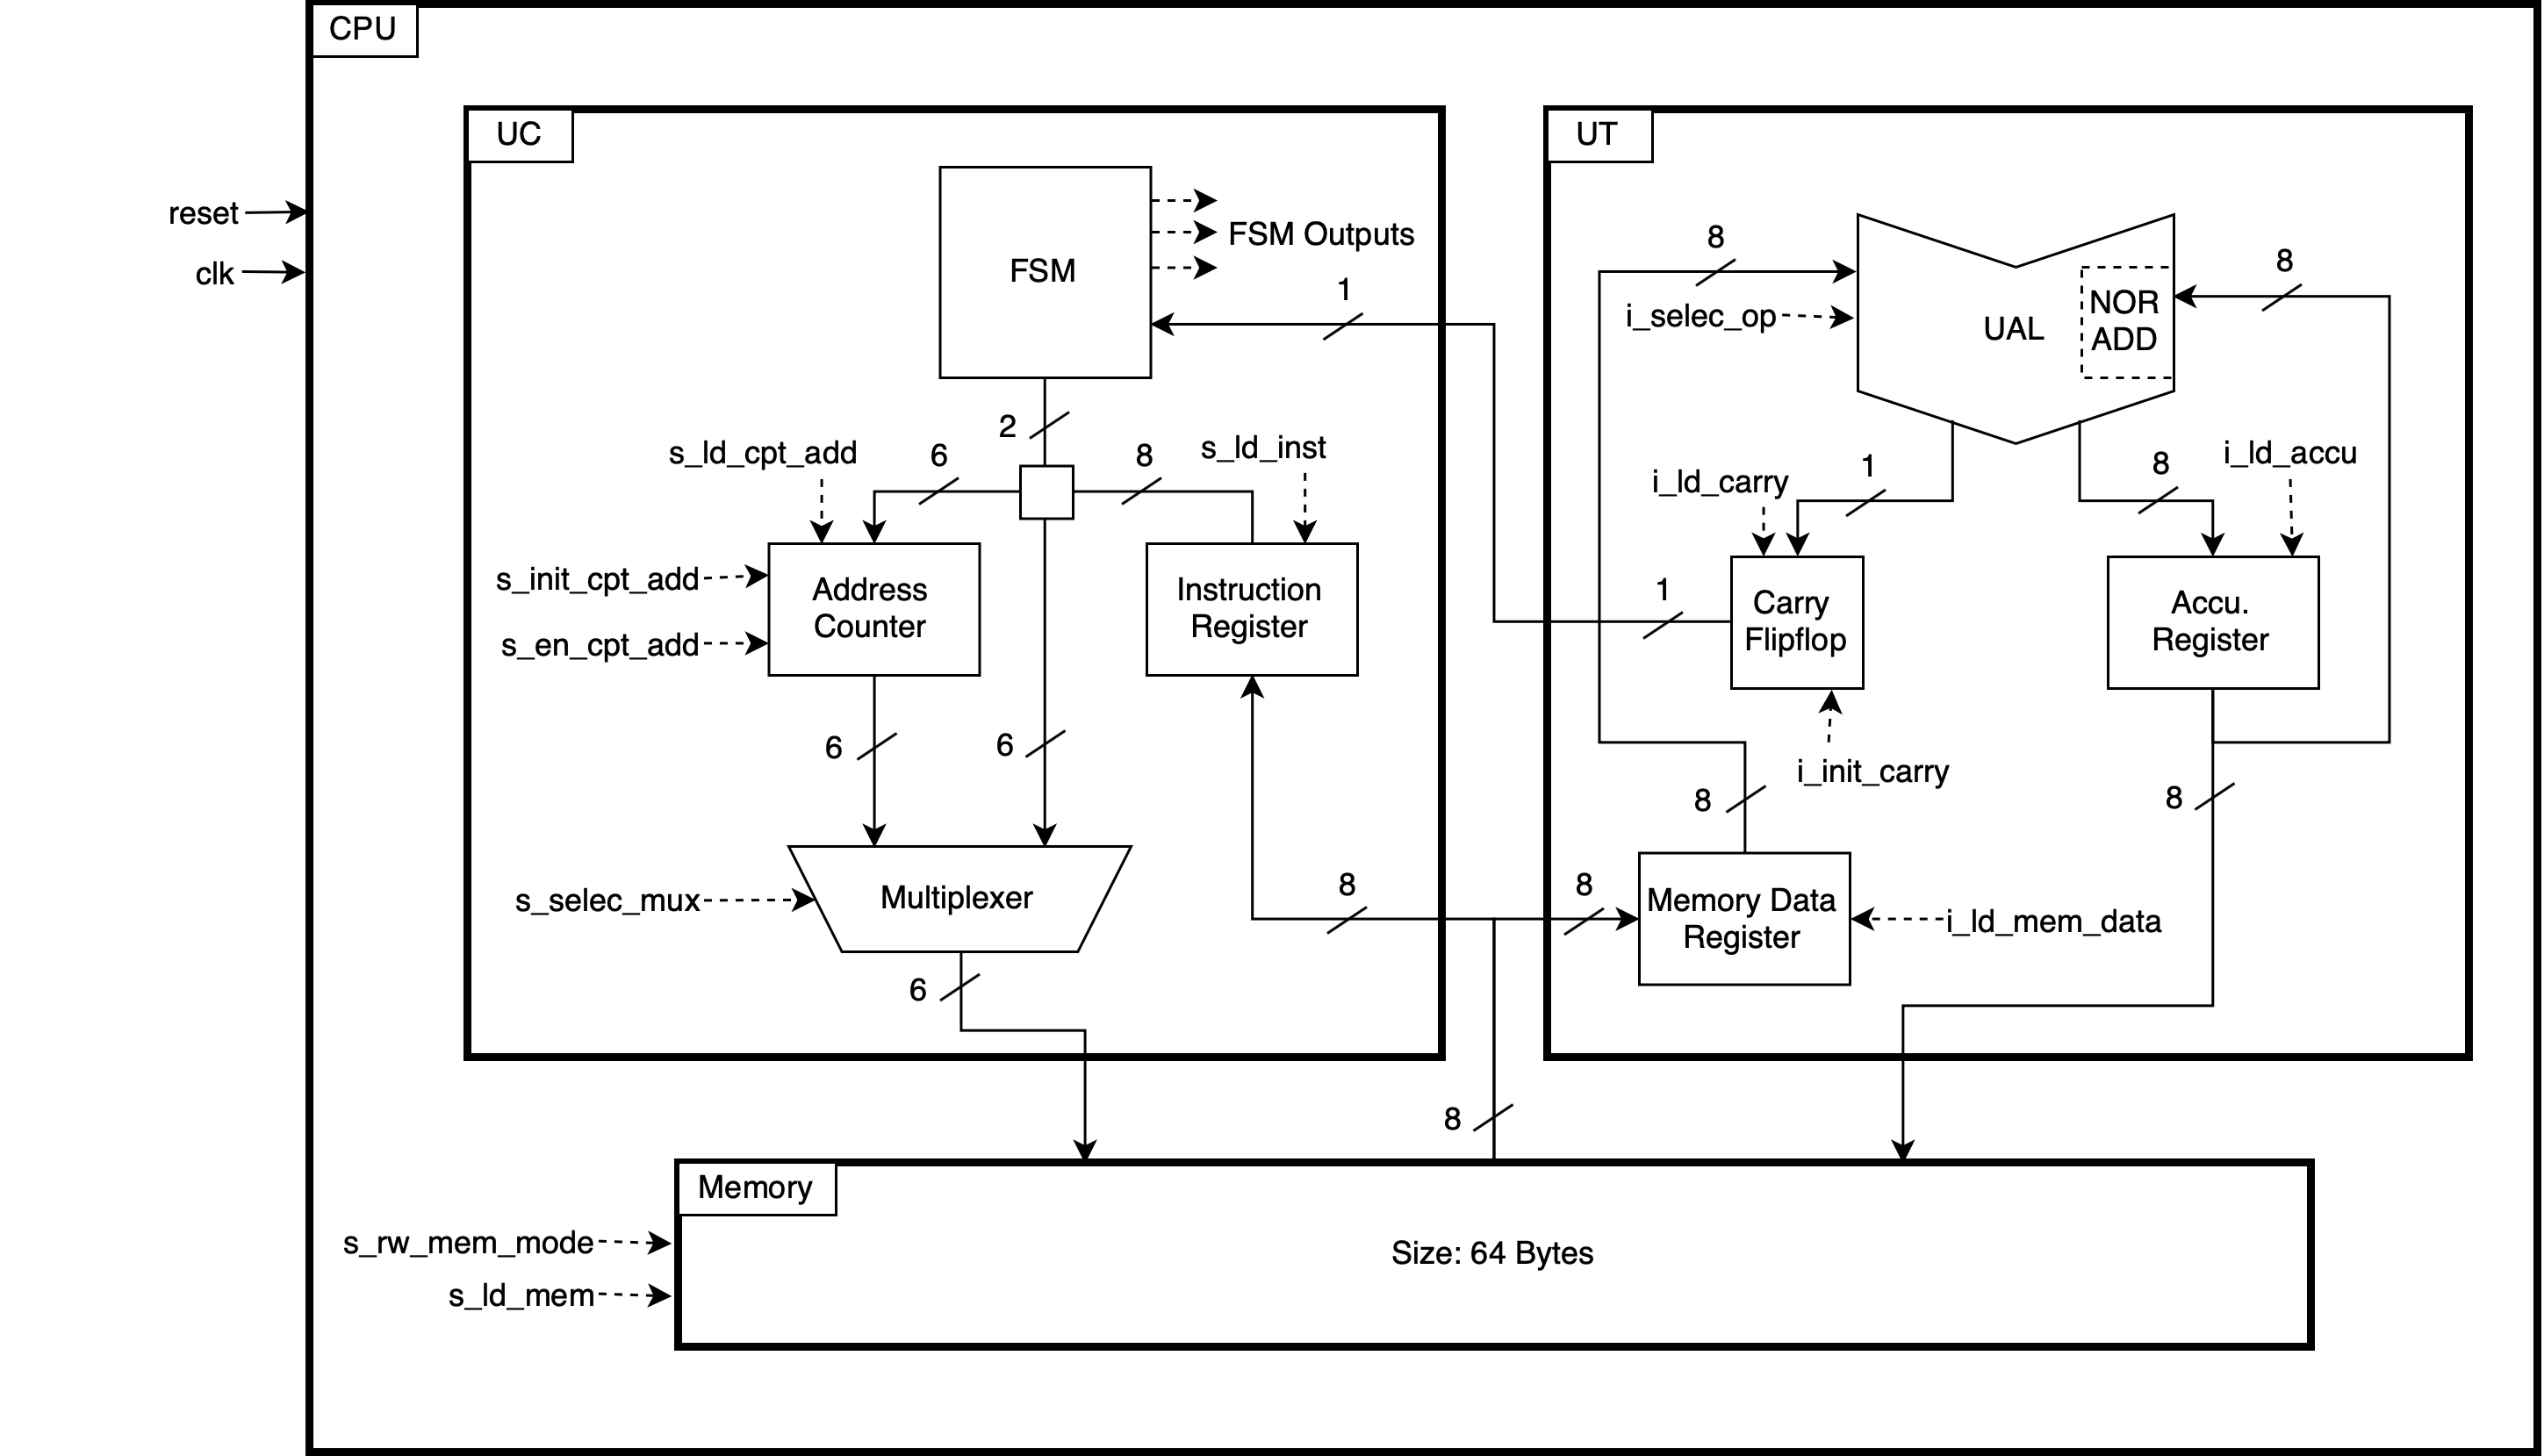
\includegraphics[width=\textwidth]{../doc/VHDL_Diagram.png}
        \caption{Architecture du CPU (Clock et reset non représentés)}
        \label{fig:vhdl_diagram}
    \end{figure}
    \subsection{Contrôleur (UC)}
    \subsubsection{Registre d'instruction}
    \par Ce registre 8 bits permet de stocker l'instruction qui est actuellement traitée par le CPU. Les instructions 8 bits sont issues de la mémoire. 
    \subsubsection{Compteur d'adresse}
    \par Ce compteur permet de définir l'adresse mémoire de la prochaine instruction que devra exécuter le CPU. Un système de chargement permet de modifier la valeur courante du compteur pour permettre des sauts d'adresse (Instruction JCC). Une entrée "init" permet de remettre à 0 le compteur pour redémarrer le programme à l'adresse 0.
    \subsubsection{Multiplexeur}
    \par Le multiplexeur est un composant purement combinatoire qui permet de sélectionner la source de l'adresse mémoire à lire/écrire. Si son signal de commande est à '0', alors c'est la sortie du compteur d'adresse qui est connectée à la mémoire. Ceci permet de lire les instructions du programme. Lorsque le signal de commande est positionné à '1', ce sont les 6 bits de poids faibles qui fixent l'adresse. Ceci permet d'effectuer les accès mémoire pour la partie calcul. 
    \subsubsection{Machine d'état (FSM)}
    \par La FSM est l'ordonnanceur du CPU. Elle génère 12 signaux qui commandent les différents composants du CPU. Voici son schéma: 
    \begin{figure}[h]
        \centering
        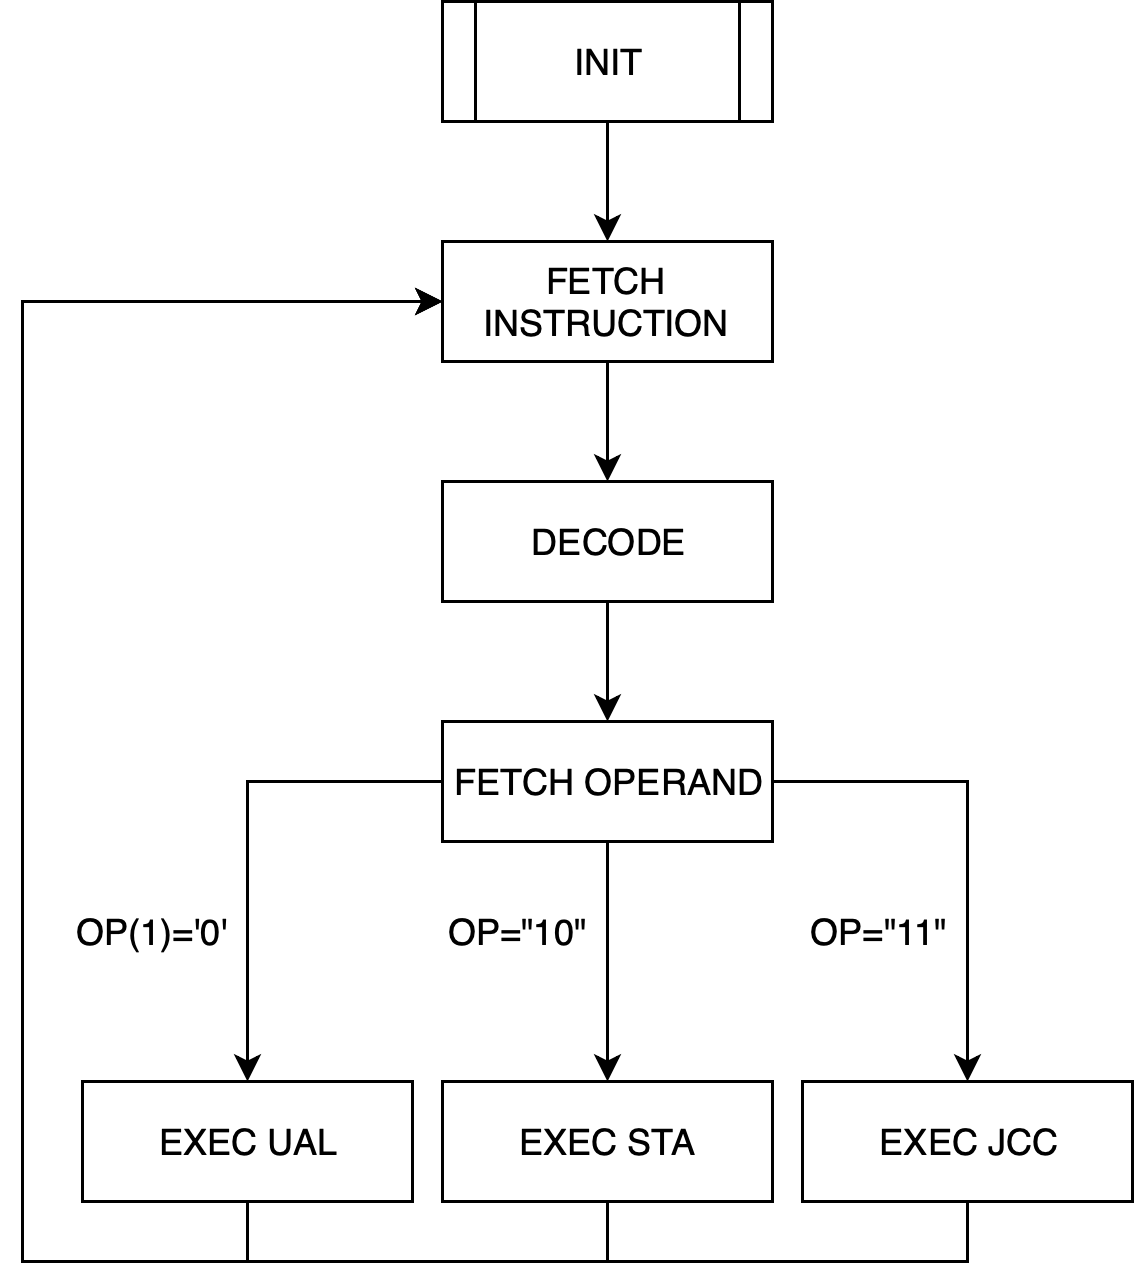
\includegraphics[width=200px]{../doc/FSMDiagram.png}
        \caption{Diagramme de la machine d'état du CPU}
        \label{fig:fsm_diagram}
    \end{figure}
    \begin{itemize}\renewcommand{\labelitemi}{$\bullet$} 
        \item INIT : Phase d'initialisation du CPU, cette étape n'est active qu'après un reset le temps d'une période d'horloge. 
        \item FETCH INSTRUCTION : Chargement de l'instruction indiquée par le compteur d'adresse.
        \item DECODE : Décodage du code opération de l'instruction et anticipation du prochain chargement de mémoire.
        \item FETCH OPERAND : Chargement de la variable pointée par l'instruction de la mémoire vers la partie opérative (UT). Le choix de l'étape suivante est conditionné par le code d'opération.
        \item EXEC UAL (Code OP = "00" ou "01") : Défini l'opération à effectuer sur la partie opérative puis ordonne la sauvegarde du résultat dans le registre d'accumulation. 
        \item EXEC STA (Code OP = "10") : Sauvegarde la valeur du registre d'accumulation en mémoire à l'adresse indiquée par l'instruction.
        \item EXEC JCC (Code OP = "11") : Effectue un test sur la valeur de la retenue pour déterminer si le saut d'adresse doit être exécuté. Le saut est effectué en plaçant les 6 bits de poids faibles de l'instruction dans le compteur d'adresse grâce au système de chargement évoqué précédemment.
    \end{itemize}
    \subsection{Contrôleur (UT)}
    \subsubsection{Registre de donnée mémoire}
    \par Ce registre permet de stocker la dernière valeur lue en sortie de la mémoire. Il est directement lié à l'unité de calcul UAL.
    \subsubsection{Registre d'accumulation}
    \par Ce registre 8 bits stocke le résultat de la partie UAL. Sa valeur peut être envoyée vers la mémoire pour être sauvegardée ou bien réutilisée pour le calcul suivant.
    \subsubsection{Unité de calcul (UAL)}
    \par Cette unité de calcul combinatoire dispose d'une entrée de sélection d'opération entre l'addition et le Non-OU. L'opération selectionnée est appliquée entre les deux valeurs 8 bits placées en entrée et le résultat est retourné vers le registre d'accumulation. Une seconde sortie permet de récupérer la retenue sur 1 bit pour être dirigée vers la flipflop. Notons que cette retenue n'est pas conservée après l'exécution d'une opération NOR.
    \subsubsection{Flipflop de retenue (Carry)}
    \par Cette bascule de type flipflop permet de stocker l'état de la retenue du dernier calcul de l'UAL. Sa sortie est utilisée par la FSM pour déterminer si le saut d'adresse de l'instruction JCC doit être effectué ou ignoré.
    \subsection{Mémoire}
    \par Cette mémoire de 64 octets est une mémoire simple accès avec un port de lecture et un second d'écriture. Elle est adressée sur 6 bits et manipule des valeurs sur 8 bits.
    \subsection{Signaux communs}
    \par Nous utilisons 3 signaux communs à tous nos composants sequentiels. L'horloge "clk" est le signal sur lequel tous les process réagissent. Sur la carte Nexys 4, cette horloge est définie à 100MHz. Pour diminuer la fréquence de fonctionnement de notre système, nous utilisons un  système de clock enable. De ce fait, nous sommes parfaitement synchrone avec l'horloge principale. Enfin, nous avons implémenté un reset synchrone qui permet d'initialiser notre CPU. 
    \par Notons toutefois que la mémoire ne dispose pas de reset. En effet, le seul moyen de réinitialiser cette mémoire est d'écrire les octets un à un de manière adressée. Il n'y a donc pas de solution pour faire cela avec un signal reset.
    
	\section{Tests}
    \par Chaque composant a été testé indépendemment à l'aide de "testbench". Une fois fonctionnels, nous les avons implémentés dans le top level nommé "CPU". Pour valider le projet, nous avons codé les deux programmes de test vu en cours dans des fichiers "*.data". Ces fichiers sont chargés dans la mémoire juste avant la simulation. En observant les derniers accès mémoire du programme, on observe que les résultats sont cohérent avec les valeurs attendus.
    \subsection{Additionneur N-bits}
    \begin{figure}[h]
        \centering
        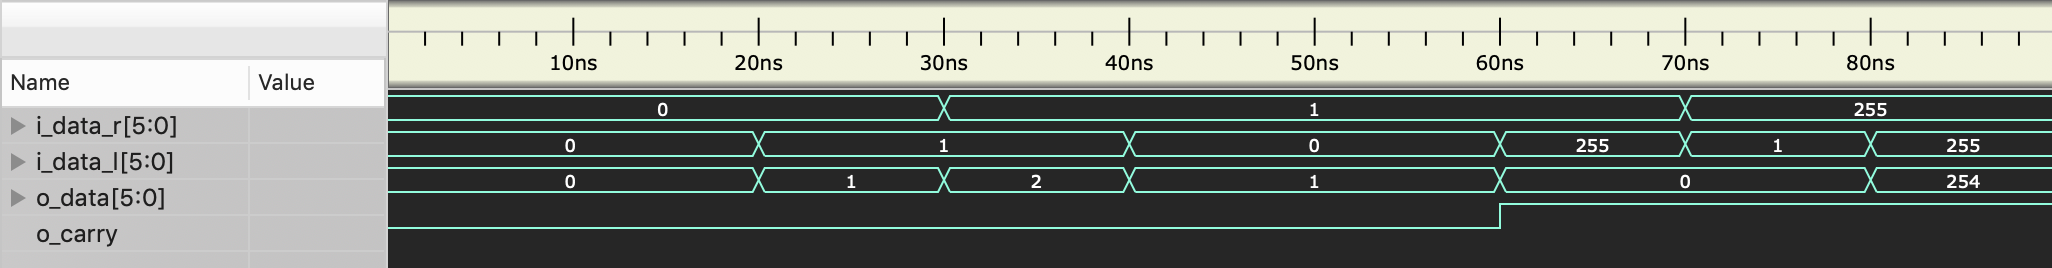
\includegraphics[width=\textwidth]{../doc/tb_screen/addi_n_bits.png}
        \caption{Diagramme temporel de l'additionneur N-bits}
        \label{fig:diag_tb_addi_n_bits}
    \end{figure}
    \par Sur cette figure, on observe que les données "right" et "left" sont additionnées en sortie. On remarque que la carry est bien mise à '1' lorsque le résultat dépasse un codage sur 8 bits.

    \subsection{Flipflop}
    \begin{figure}[h]
        \centering
        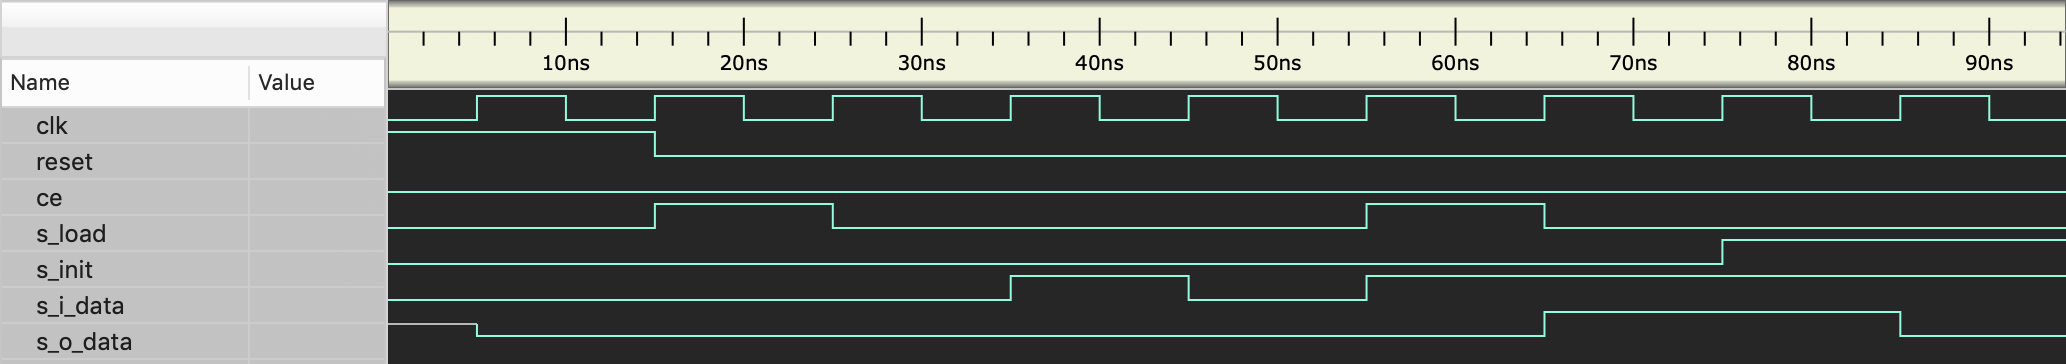
\includegraphics[width=\textwidth]{../doc/tb_screen/flipflop.png}
        \caption{Diagramme temporel de la flipflop de retenue}
        \label{fig:diag_tb_flipflop}
    \end{figure}
    \par Ici nous avons un premier "load" qui recopie le '0' de "i\_data" vers la sortie puis un changement sur "i\_data" pour montrer que la sortie n'évolue pas sans la présence du signal "i\_load". Enfin, nous avons un changement de la sortie à '1' de par la présence du chargement et du '1' en entrée. La bascule est finalement reset par le signal "s\_init".

    \subsection{Multiplexeur à 2 entrées}
    \begin{figure}[h]
        \centering
        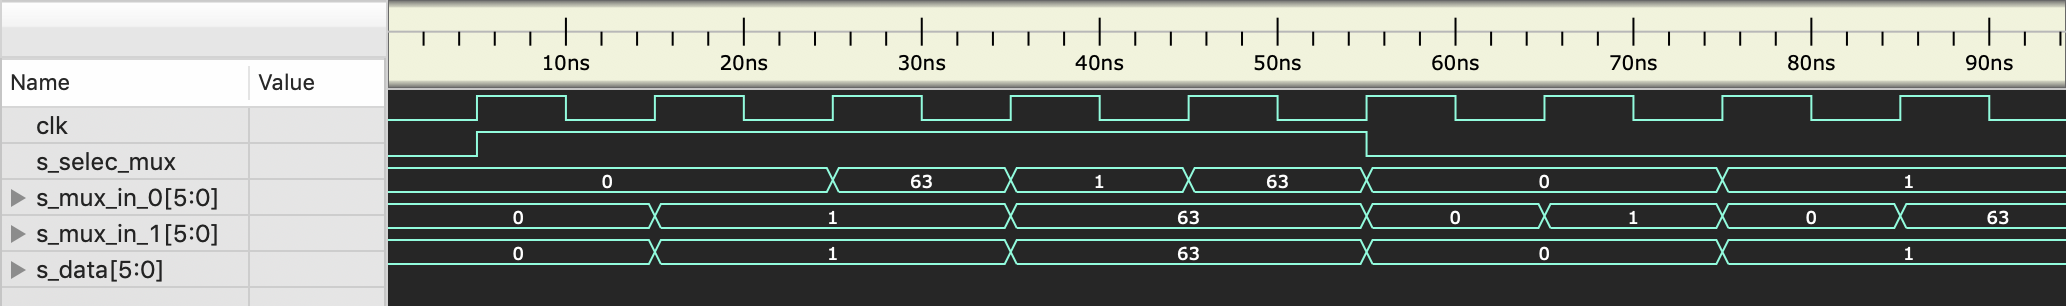
\includegraphics[width=\textwidth]{../doc/tb_screen/mux_2_in.png}
        \caption{Diagramme temporel du multiplexeur}
        \label{fig:diag_tb_mux_2_in}
    \end{figure}
    \par Cette figure nous montre que les signaux "s\_mux\_in\_0" et "s\_mux\_in\_1" évolue en fonction du temps avec des valeurs sur 6 bits. Les valeurs extrêmes sont utilisées pour les biens du testbench. Le signal "s\_selec\_mux" permet de choisir quelle entrée recopier en sortie.

    \subsection{Unité de calcul}
    \begin{figure}[h]
        \centering
        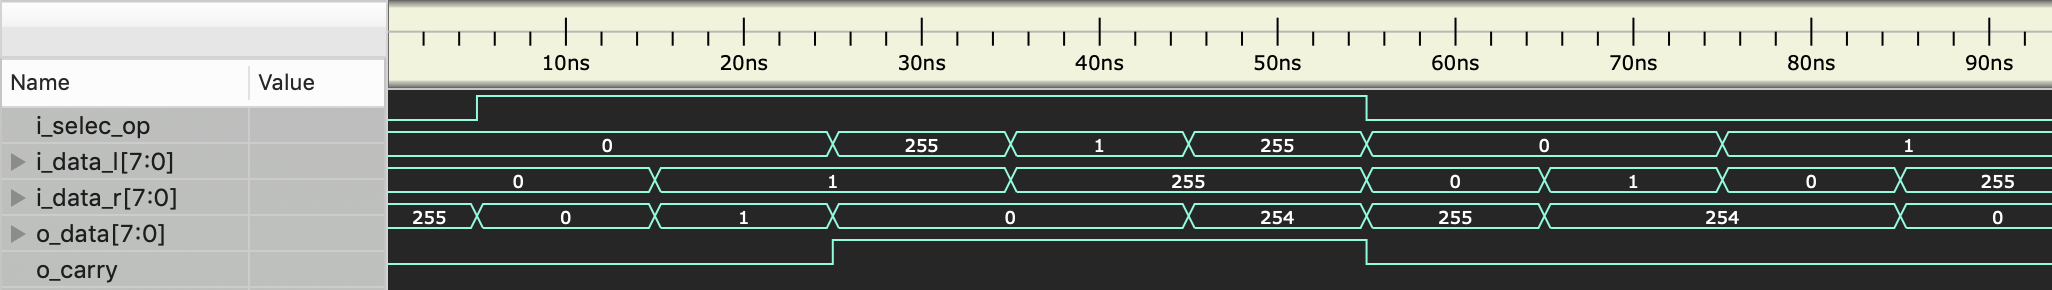
\includegraphics[width=\textwidth]{../doc/tb_screen/ual.png}
        \caption{Diagramme temporel de l'unité de calcul UAL}
        \label{fig:diag_tb_ual}
    \end{figure}
    \par L'UAL dispose de deux opérations. L'addition a été testée dans un premier temps en définissant "i\_selec\_op" à '1' puis le Non-OU dans un second temps. Une fois de plus les entrées "left" et "right" prennent des valeurs spécifiques pour tester les limites du système.
    \par On observe en premier lieu que la sortie est bien la somme des entrées avec la mise à jour de la retenue. Puis nous constatons que l'opération NOR fonctionne aussi.
    
    \subsection{CPU - Programme du PGCD}
    \begin{figure}[h]
        \centering
        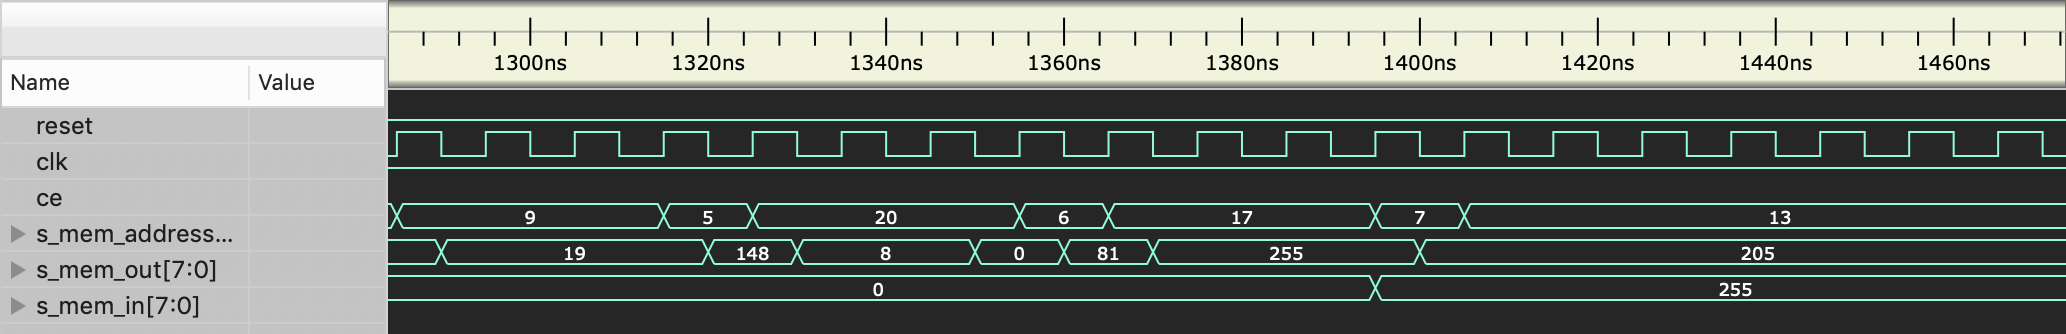
\includegraphics[width=\textwidth]{../doc/tb_screen/cpu_2nd_prog.png}
        \caption{Diagramme temporel du CPU avec programme de PGCD}
        \label{fig:diag_tb_cpu_2nd_prog}
    \end{figure}
    \par Ce diagramme a été obtenu en combinant tous les blocs précédents. Il montre les accès mémoire lorsque le programme de calcul de PGCD arrive à sa fin. On observe que le signal "s\_mem\_out" passe de 8 à 0 aux alentours de 1340ns. Ceci correspond à la dernière opération effectuée sur la variable 'a' à la fin de l'algorithme lorsque 'a' est soustrait pour la dernière fois. Les données de départ étant 40 et 24, notre résultat de 8 est donc cohérent.  

    \subsection{FSM}
    \begin{figure}[h]
        \centering
        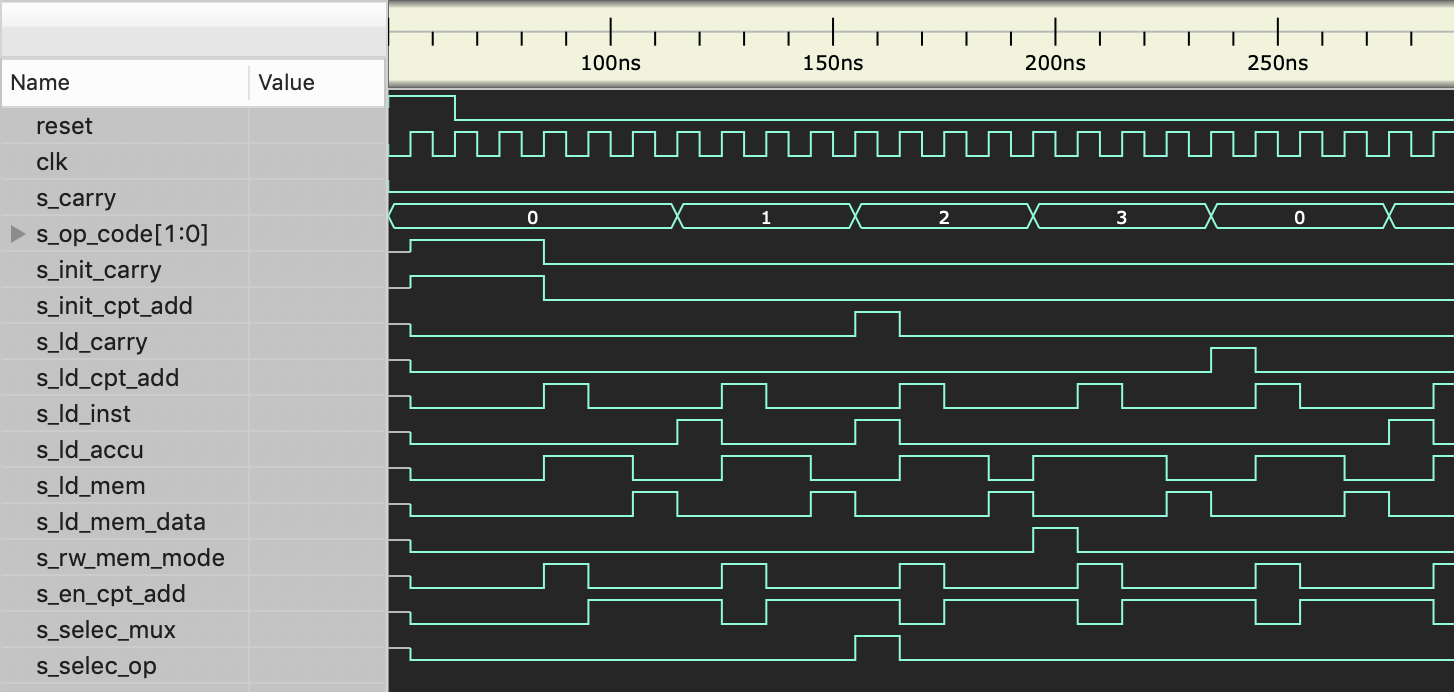
\includegraphics[width=\textwidth]{../doc/tb_screen/fsm.png}
        \caption{Diagramme temporel de la FSM}
        \label{fig:diag_tb_fsm}
    \end{figure}
    \par Ce diagramme temporel nous montre l'évolution des signaux de sortie de la FSM en fonction des instructions reçues par le CPU. On remarque clairement que chaque instruction est exécutée en 4 périodes d'horloge.

    \newpage
    \subsection{Interfacage pour test sur carte}
    \par Pour tester notre CPU, nous avons récupéré le composant "acces\_carte". Cette interface nous impose de sortir notre bus de donnée et notre valeur d'adresse courante pour pouvoir les visualiser sur la carte de dévelopement.
    \par Ces deux composants sont associés dans un Top Level qui inclue une PLL pour générer une horloge de 25MHz à partir de l'horloge principale de 100MHz. Ce signal est envoyé sur l'interface pour générer des signaux de plus basse fréquence que nous connectons à l'entrée "clock enable" de notre CPU. Ceci nous permet d'observer l'évolution des accès mémoire sur l'écran 7-segments. Pour que le résultat soit affiché à la fin du programme de PGCD, nous avons ajouté deux instructions avant la boucle infinie pour faire en sorte que la valeur "b" soit chargée dans le registre d'accumulation. Voici ce que nous obtenons :
    \begin{figure}[h]
        \centering
        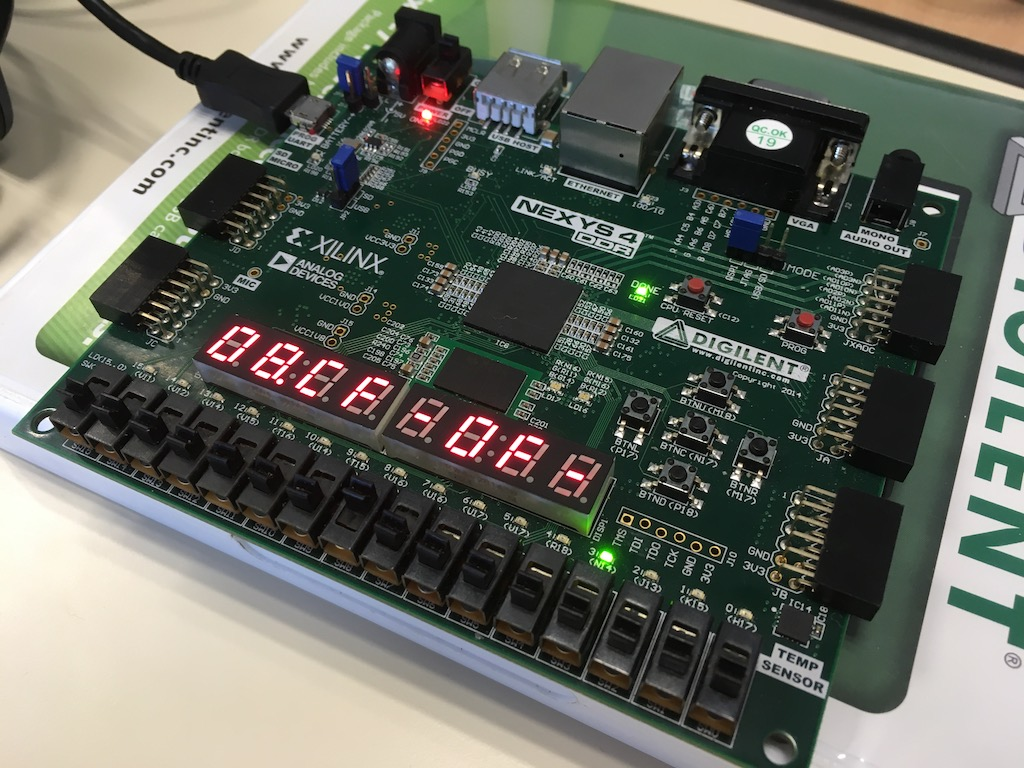
\includegraphics[width=\textwidth]{../doc/photo/resultat_test_pgcd.jpeg}
        \caption{Résultat de notre programme PGCD sur la Nexys4 DDR}
        \label{fig:resultat_test_pgcd}
    \end{figure}
    \par Dans l'ordre, nous avons 0x08 qui indique la valeur de notre registre d'accumulation (ici le résultat du PGCD), 0xCF est l'instruction qui est en cours d'exécution, ici un JUMP à l'adresse 15 pour la boucle infinie. Enfin, 0x0F est l'adresse de l'instruction qui va être exécutée.
    \newpage

    \section{Conclusion}
    \par Ce projet nous a fait découvrir les fonctionnements internes d'un processeur ainsi que les problématiques d'accès mémoire. L'implémentation en VHDL nous a permis de se remémorer les bonnes pratiques des langages de description. De plus, la réutilisation des nos anciens composants VHDL nous a montré qu'il était important de bien structurer et bien documenter nos fichiers pour être plus efficace dans nos futurs projet.

    % =====================
    % BACK MATTER
    % =====================
\end{document}